\chapter{Related Work}
\label{cha:relatedwork}

\section{Human Mobility within the city}
\label{cha:introduction_hummob}

According to research \cite{HumanMobility1}\cite{HumanMobility2}\cite{HumanMobility3}, the average walking speed in the city for man aged 40 is 1.4 m/s (5 km/h), and slowest one is for elderly (with walking impairment) below 1 m/s (3.6 km/h). 

TODO: elaborate a bit more

\section{Approaches to stop detection for localization services}
\label{cha:introduction_appr_stopdet}

\subsection{Stop Detection analyzing repetitive appearance at location}

\subsection{Stop Detection based on continuous localization}

\subsection{Stop Detection based on mobility index}
\label{cha:introduction_mob_index_sect}

In the paper \cite{MobilityIndexGIS}, movement of mobile devices between cells (handovers) is considered. To detect the periods of slow movements of stops at the specific location, parameter called Mobility Index is considered. 
\begin{figure}[!ht]
	\centering
	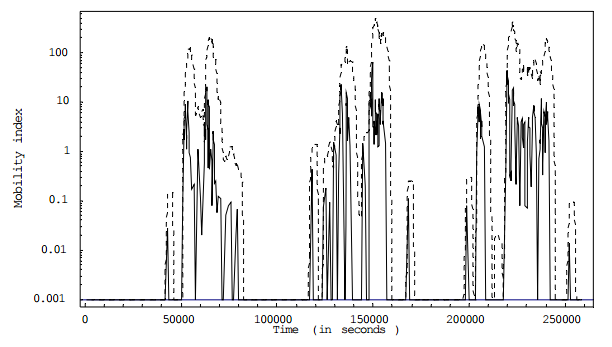
\includegraphics[width=0.5\textwidth]{images/intro_mobility_index.png}\\
	\caption{Mobility Index. Source: \cite{MobilityIndexGIS}}
	\label{fig:introduction_mob_index}
\end{figure}
\\
In a populated area, with many GSM cells, the mobile
terminal can change from one cell to another within
seconds or after several minutes. Given a set of consecutive records, the mobility of a user can be estimated by calculating the Mobility Index over a pre-defined time period (sliding window). The Mobility Index is defined as the sum of the "distances" between each record and the previous ones, where the "distance" is the inverse of the time spent on each cell. If the value of MI is below certain threshold, it is assumed that the object stopped or moved slowly. In the publication, sliding window of 10 minutes and a mobility index threshold value of 6 has been used for certain area. The obtained results were in agreement with actual movements during more than 90\% of the time. 
\\\\
Rapid drop in mobility index represents a set of points (restricted area) in which user has been moving slowly or stopped. Slight decrease in mobility index means that user changed position from restricted area and is moving.
\section{Use of graphical analysis in networks}
Use of graphical analysis of data is a very common practice in many areas of scientific research. Representing human movement behavior as network allows us to easily visualize the data as well process it using various data mining algorithms. Here we present some examples of graphical analysis used in various fields of research. 
\subsection{Algorithms for graphical analysis} 
Some of the most commonly used algorithm used for graphical analysis of data are: PageRanks, Degree distribution, connected components, triangle count.
\cite{kelly2008mathematics} discusses the concept of link-route incidence matrix where columns of the matrix corresponds to routes, and rows to the links of the network. The link-route incidence matrix has been used in predicting the number of routes between two nodes.
\subsection{Graphcal analysis for computer networks}
Graph based approach is implemented in case of analysis computer networks and the Internet. As we can see from \cite{djidjev2011graph} \cite{deri2013graph} graphical representation and analysis has been implemented for studying network traffic and DNS flow request. 

In \cite{djidjev2011graph} we see that subgraphs based on user behavior is extracted from the main larger graph to analyze traffic pattern and identify malicious behavior. In this paper, Djidjev, Sandine et al. have useed the SSH flow records to create a directed multigraph, where node set represents hosts and servers and edges represent SSH sessions. 

As we see in \cite{deri2013graph} three different bipartite graphs are used to model the DNS resolvers, domains and their interactions. In this paper, Deri,Mainardi et al. have used the concept of adjacency to determine common neighbors between two DNS domains. 
\subsection{Graphical analysis for human social network}
\subsection{Graphical analysis ab in transport network}
\cite{marzuoli2011two} discussed a two step based process for building the network graph based on air traffic. In their study, Marzuoli et al. have used the concept of graph theory to create a network flow model of the Airspace. They define their network as a system of nodes and directed edges. Working with air traffic, they defined network nodes as areas where aircraft are entering, leaving a region and edges as flow corridors used by the aircrafts. Next, they use the concept of origin-destination matrices by creating origin-destination pairs out of their data to determine relative importance of origin-destination pairs or routes used by aircrafts.
